\documentclass{tu_coursework}

%================================================================================
% МЕТАДАННИ
\title{Боен робот с пулт за дистанционно управление по радио връзка}
\doctype{ДИПЛОМНА РАБОТА}
\author{Александър Иванов}
\speciality{Системно програмиране}
\admgroup{69}
\faculty{ТЕХНОЛОГИЧНО УЧИЛИЩЕ ЕЛЕКТРОННИ СИСТЕМИ\\ към ТЕХНИЧЕСКИ УНИВЕРСИТЕТ - СОФИЯ}
\fac{ФЕТТ}
\facnumber{101218420}
\supervisor{инж. Владимир Гаристов}
% Закоментирай долния ред, ако няма рецензент
\reviewer{проф. д.т.н. Юлиан Вучков}
\date{\today}
\city{София}



\begin{document}

%================================================================================
% Заглавие
\maketitle
\cleardoublepage

%================================================================================
% Задание

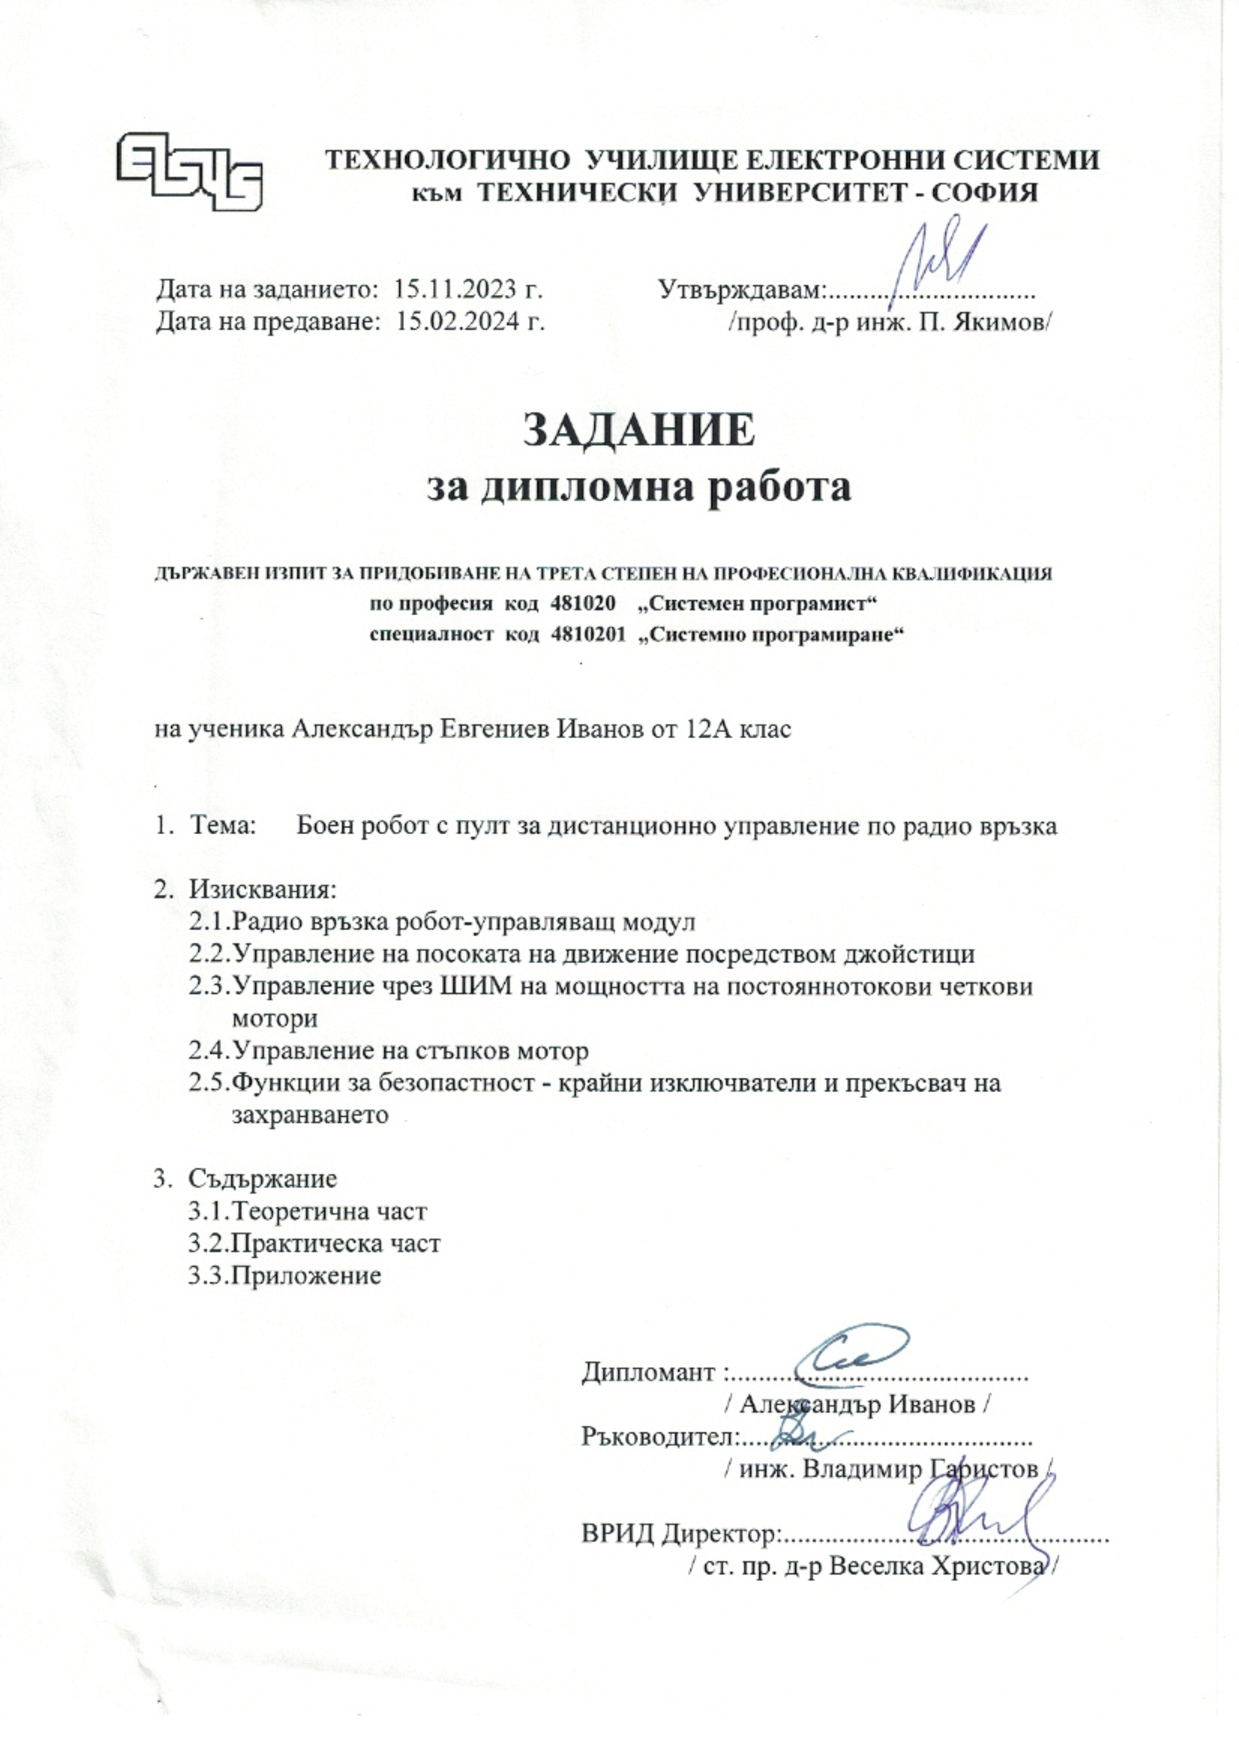
\includepdf[pages={1}]{documents/assignment_signed.pdf}
\pagenumbering{arabic}

%================================================================================
% Глави

\chapter{Увод}
Още от зората си, човечеството търси разнообразни и вълнуващи начини да успее да избяга от еднообразното си ежедневие. За целта много и различни методи за развлечение са възникнали, вариращи от приятелски игри до зрелищни спектакли. Едно от най-разпространените забавления още от тогава е също толкова популярно и днес, а именно – боевете. Зрелището на това два индивида да се бият помежду си завладява всеки зрител. Годините са доказали, че колкото по-драматична е една битка, толкова по-силни са чувствата, които се пораждат у нейните наблюдатели. Но това води до един неизбежен проблем: участниците в такива интензивни битки винаги биват физически наранени. Поради тази причина се появява казусът как може да се постигнат тези зрелища, без участниците да пострадат. Решението на този проблем са битките с бойни роботи (или батълботи). Стандартна битка трае 3 минути и в тях роботизираните системи, контролирани с дистанционно управление, целят увреждането на опонента до такава степен, че вече да не може да извършва движения.


\chapter{ Методи, средства и методологии за изработване на бойни роботи}

%================================================================================
% ЗАДВИЖВАНЕ

\section{Основни методи и технологии за задвижване на бойни роботи}
\label{sec:motion-types}

Бойните роботи традиционно могат да се задвижват по три начина чрез вериги, колела или механични крака. Има и други начини, но те не са ефективни в битка.
Роботите, задвижвани с танкови вериги, имат отлично сцепление със земята и вървят много стабилно, но имат много недостатъци. Поради голямата площ на триене при завъртане те изразходват значително количество енергия. Освен това и самото движение се извършва сравнително бавно, което позволява на опонента да заобиколи робота и да го удари в гръб. Боен робот, задвижван от верига, може да се види на \cref{fig:using-treads}.

\begin{figure}[H]
    \centering
    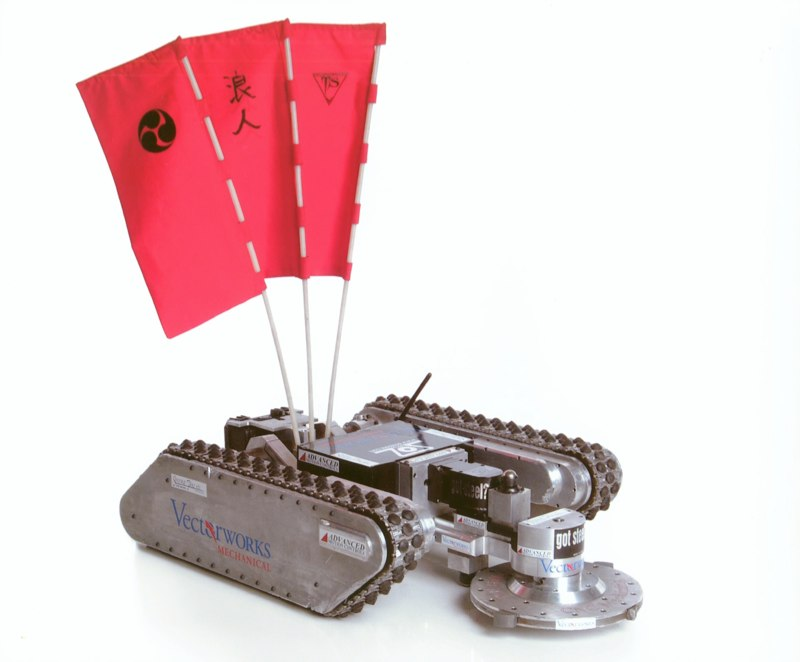
\includegraphics[width=0.5\linewidth]{images/using-treads.jpg}
    
    \caption{Боен робот, задвижван от вериги}
    \label{fig:using-treads} 
\end{figure}

Механичните крака имат също много недостатъци. Някои от които са, че са много сложни за конструкция и контрол. Друг техен недостатък е, че те не са достатъчно здрави по време на битка, особено срещу посичащите спинер роботи. Повече за този тип бойни роботи може да се прочете в \cref{sec:robot-types}. Трета слабост е, че центъра на тежестта на роботи с такава система за задвижване е много високо над земята, което ги прави уязвими срещу атаки, целящи преобръщане. Батълбот, използващ механични крака може да бъде видян на \cref{fig:using-legs}.

\begin{figure}[H]
    \centering
    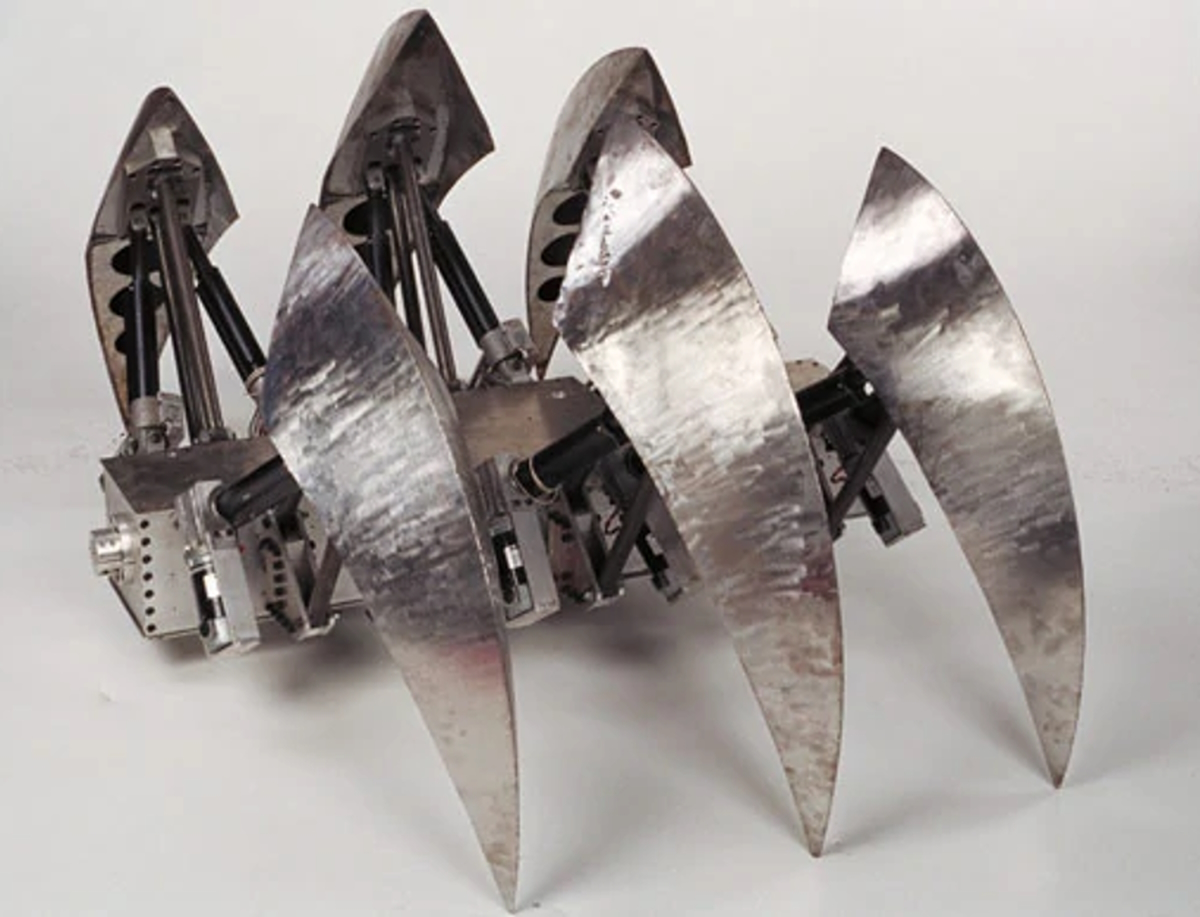
\includegraphics[width=0.6\linewidth]{images/using-legs.jpg}

    \caption{Боен робот, задвижван от механични крака}
    \label{fig:using-legs} 
\end{figure}

Поради гореспоменатите причини, най-често бойните роботи се задвижват чрез колела. Разпространени са два начина на управление на задвижването на моторни средства с колела – Акерман управление и диференциално управление. Акерман управлението е възприето от повечето моторни-превозни средства. При него един голям мотор задвижва колелата и един по-малък отговаря за тяхното завъртане. То е ефективно при движение в права линия, но когато трябва да се завие се изискват определени маневри. Диференциалното управление е много по-често срещано в роботиката. При него лявата и дясната страна на робота се задвижват напълно индивидуално. Недостатъкът на този метод е фактът, че за да се движи моторното средство в права линия двете половини требва да имат еднаква скорост, което е трудно за постигане. Голямото преимущество обаче е, че завиването става значително по-бързо.

Освен по начин на управление на задвижването роботите придвижващи се с колела се различават помежду си и чрез броя на задвижваните колела. При такива с две задвижващи колела и диференциално управление на задвижването, завиването се случва със сравнително ниски загуби на енергия. Проблемът е, че с две опорни точки, роботът най-вероятно ще има нужда от поне още една такава. Той се решава чрез добавянето на ball transfer units.


%================================================================================
% КОМУНИКАЦИЯ

\section{Основни методи и технологии за дистанционно управление на бойни роботи}

Съгласно официалните изисквания за работа към бойните роботи, те трябва да бъдат контролирани безжично дистанционно. За целта могат да се използват много технологии за безжична комуникация, като едни от най–популярните са Wi-Fi, Bluetooth и nRF24L01.

Wi-Fi позволява много висока скорост на предаване на информацията, но има много недостатъци. Един от тях е, че има много високо потребление на енергия. Друг е, че не може директно да се предава информация от едно устройство на друго безжично, а първо трябва тази информация да се подаде на маршрутизатор и след това той да я изпрати до устройството получател. Отделно по време на боевете се очаква да има голяма публика и безплатен Wi-Fi което предполага, че каналите, които се използват за тази технология ще бъдат претоварени и съответно ще има по-лоша свързаност. 

Bluetooth технологията осигурява средна скорост на предаване на информация, на цената на средно ниво на консумация на енергия. Недостатъкът е, че за да могат две устройства да се свържат и да общуват безжично и двете трябва предварително да се сдвоят, което е непрактично за системи, които не включват компютри или телефони.

Модулът nRF24L01 позволява безжична радиочестотна комуникация с други такива модули. От трите технологии за безжична комуникация този модул предлага тази с най-ниско потребление на енергия. За разлика от Wi-Fi, nRF24L01 може да се комуникира с друго устройство директно, без необходимостта от маршрутизатор. Предимството му пред Bluetooth е, че не е необходимо предварително двете устройства да се сдвояват.

\begin{table}[H]
    \centering
    \begin{tabular}{| m{4cm} | m{3,5cm} | m{3,5cm} | m{3,5cm} |}
        \hline
        & Wi-fi & Bluetooth & nRF24L01+ \\
        \hline
        Скорост &  Висока & Средно & Средна \\
        \hline
        Обхват & 10ки метри & 10 метра & 10-150 метра \\
        \hline
        Енергийна консумация & Висока & Средна & Ниска\\
        \hline
    \end{tabular}
    \caption{Сравнителна таблица за безжични технологии}
    \label{table:wireless}
\end{table}


%================================================================================
% БРОНЯ

\section{Основни методи за защита на бойни роботи}

За защита на бойните роботи винаги се монтира броня около неговата структура. Видовете броня са: традиционна, аблативна и реактивна.

Традиционната броня е изработена от много здрави и твърди материали, които се стремят да абсорбират и предадат енергията на удара без да се повреждат. Високата твърдост и здравина на този вид защита често се използва за чупене или изтъпяване на остриетата на вражеските оръжия и запазване целостта на робота при удари. Благодарение на здравината си тази броня по-рядко трябва да се сменя след битки, но нейният недостатък е, че при удар енергията на сблъсъка се предава до елементите вътре в робота, което може да доведе до тяхното повреждане.

Аблативната защита, от друга страна е проектирана да предпазва от щети робота, като самата тя бива повреждана чрез процеса аблация. Това е процеса на премахване на материал от повърхността на обект посредством изпарение или стружко отделяне. Материалите, от които е изградена са също твърди и здрави, но за разлика от традиционната броня имат по-ниска твърдост. Поради това тяхно свойство, когато тези брони трябва да предпазват от силни удари, вътрешните елементи биват изложени на риск. Материали като дървото са много ефикасни представители на този вид елементи, но друг техен недостатък е, че сблъсъците водят до много визуални следи, което често носи допълнителни точки на опонента за щети.

Третия вид броня е реактивната. По време на удар тя реагира по някакъв начин, за да предотврати щети. Има различни видове реактивна броня и всяка има свой предимства и недостатъци. Пример за такъв вид защита е пласт гума между два пласта метал. Предимството й е, че в случай на удар, пластът гума би абсорбирал енергията на удара. Този вид броня не е ефективна в боевете с роботи, поради причината, че много бързо бива повреждана и спира да пази.

%================================================================================
% ВИДОВЕ РОБОТИ

\section{Видове съществуващи бойни роботи}
\label{sec:robot-types}

Съществуват много различни видове батълботи. Основно изискване към всеки от тях е да имат поне едно оръжие, чрез което да могат да повредят опонента. В зависимост от своето оръжие роботите се разделят на 14 типа: „rammer“, „wedge“, „lifter“, „flipper“, „spearbots“, „horizontal spinner“, „sawbot“, „vertical spinner“, „drumbot“, „hammerbot“, „clamper“, „crusher“, „flamethrower“ и „multibot“. Има и други видове роботи, но те почти винаги могат да бъдат категоризирани в един от гореспоменатите видове. За ефективността на бойния робот в битка има голямо значение какво оръжие е избрано. Примерно със своите огромни дискове нанасящи разрушителни удари роботите с оръжие „vertical spinner“ са много ефективни срещу голяма част от роботите. Те имат обаче един фатален недостатък, който се изразява в това, че поради голямата скорост на въртене на съответното оръжие генерират жироскопичен ефект, който намалява осезателно скоростта им на движение, което ги прави уязвими към удари отзад. С времето в роботските боеве категориите „flipper“, „horizontal spinner“, „vertical spinner“, „drumbot“, „hammerbot“ и „clamper“ са се откроили като по-ефективни в сравнение с останалите.


\chapter{Дизайн и блоковата схема на робота}

\section{Функционални изисквания към робота}

\section{Блокова схема на робота}

\chapter{Механика}

%================================================================================
% ЦЯЛОСТЕН МОДЕЛ
 
\section{Цялостен модел на робота}

Както е описано в предишната глава, дизайна на бойния робот е вдъхновен от робота SawBlaze. Материала, който е използван за изграждането на прототипа на проекта е два милиметра дебела студено валцована въглеродна стомана DC01. Механичната конструкция на робота може да бъде разделена на два основни компонента - шасито, в което седят почти всички елементи, и механичната ръка, на която е закрепено оръжието.  

\begin{figure}[H]
    \centering
    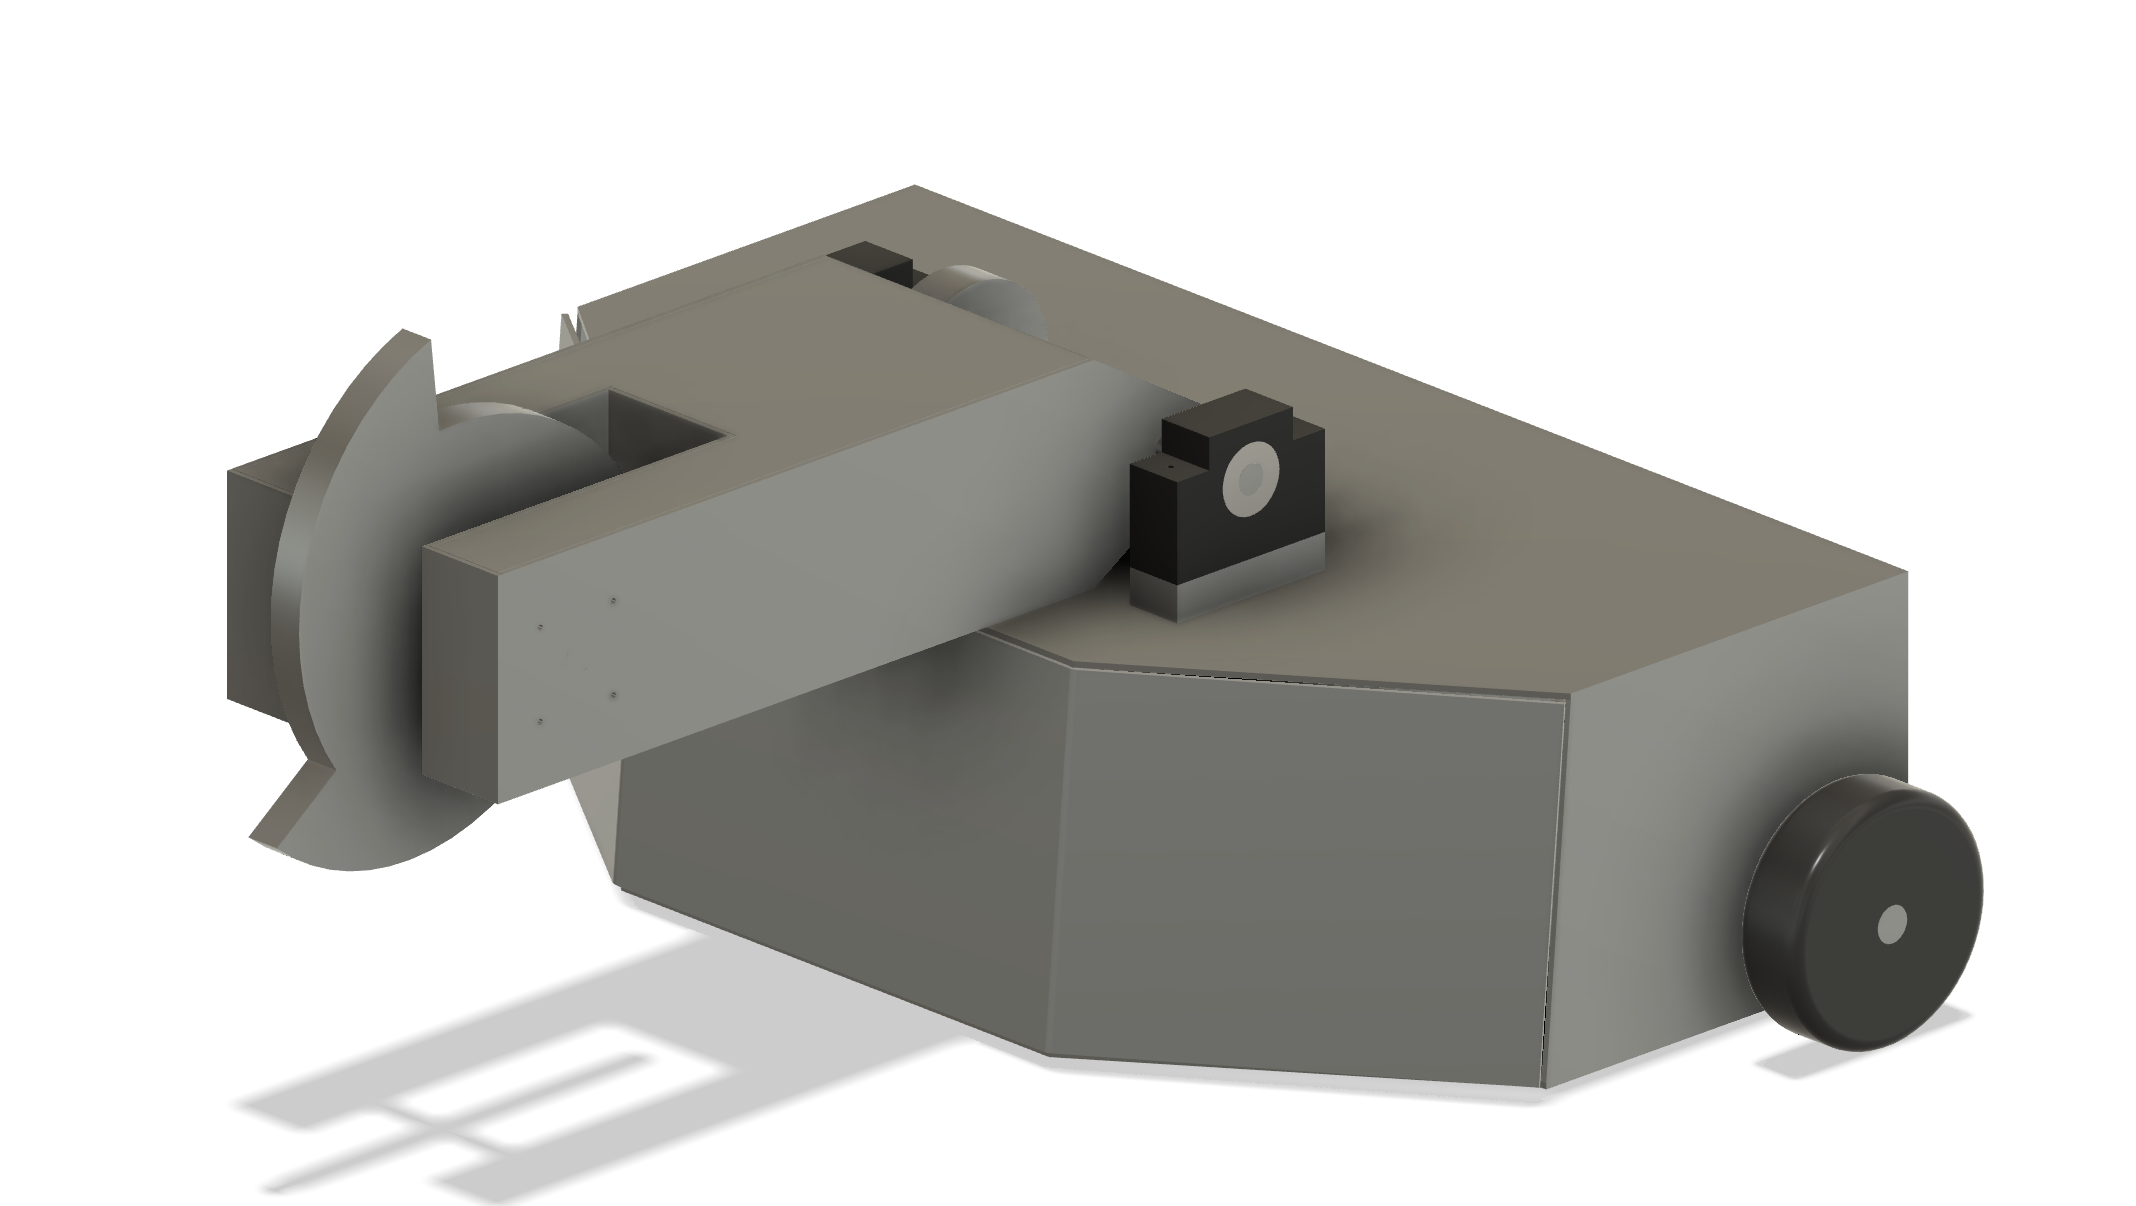
\includegraphics[width=1.1\linewidth]{images/robot-home.png}
    
    \caption{3D макет на бойния робот}
    \label{fig:robot-home} 
\end{figure}

%================================================================================
% ЗАДВИЖВАНЕ

\section{Задвижване на робота}
\label{sec:motion}

По време на проектирането на механиката на боен робот първият проблем, който трябва да бъде разгледан е как той ще се придвижва по арената. След направеното проучване в \cref{sec:motion-types} бе установено, че най-ефективният метод е диференциалното задвижване с колела. По дизайн роботът има две задвижващи колела отдвете си страни и още две допълнителни пасивни колела, които го балансират и му помагат да се движи по-добре. Всяко от задвижващите колела е с външен диаметър 80мм и ширина 12мм. Използваните мотори за тяхното задвижване са CHANCS 895 DC.

\begin{figure}[H]
    \centering
    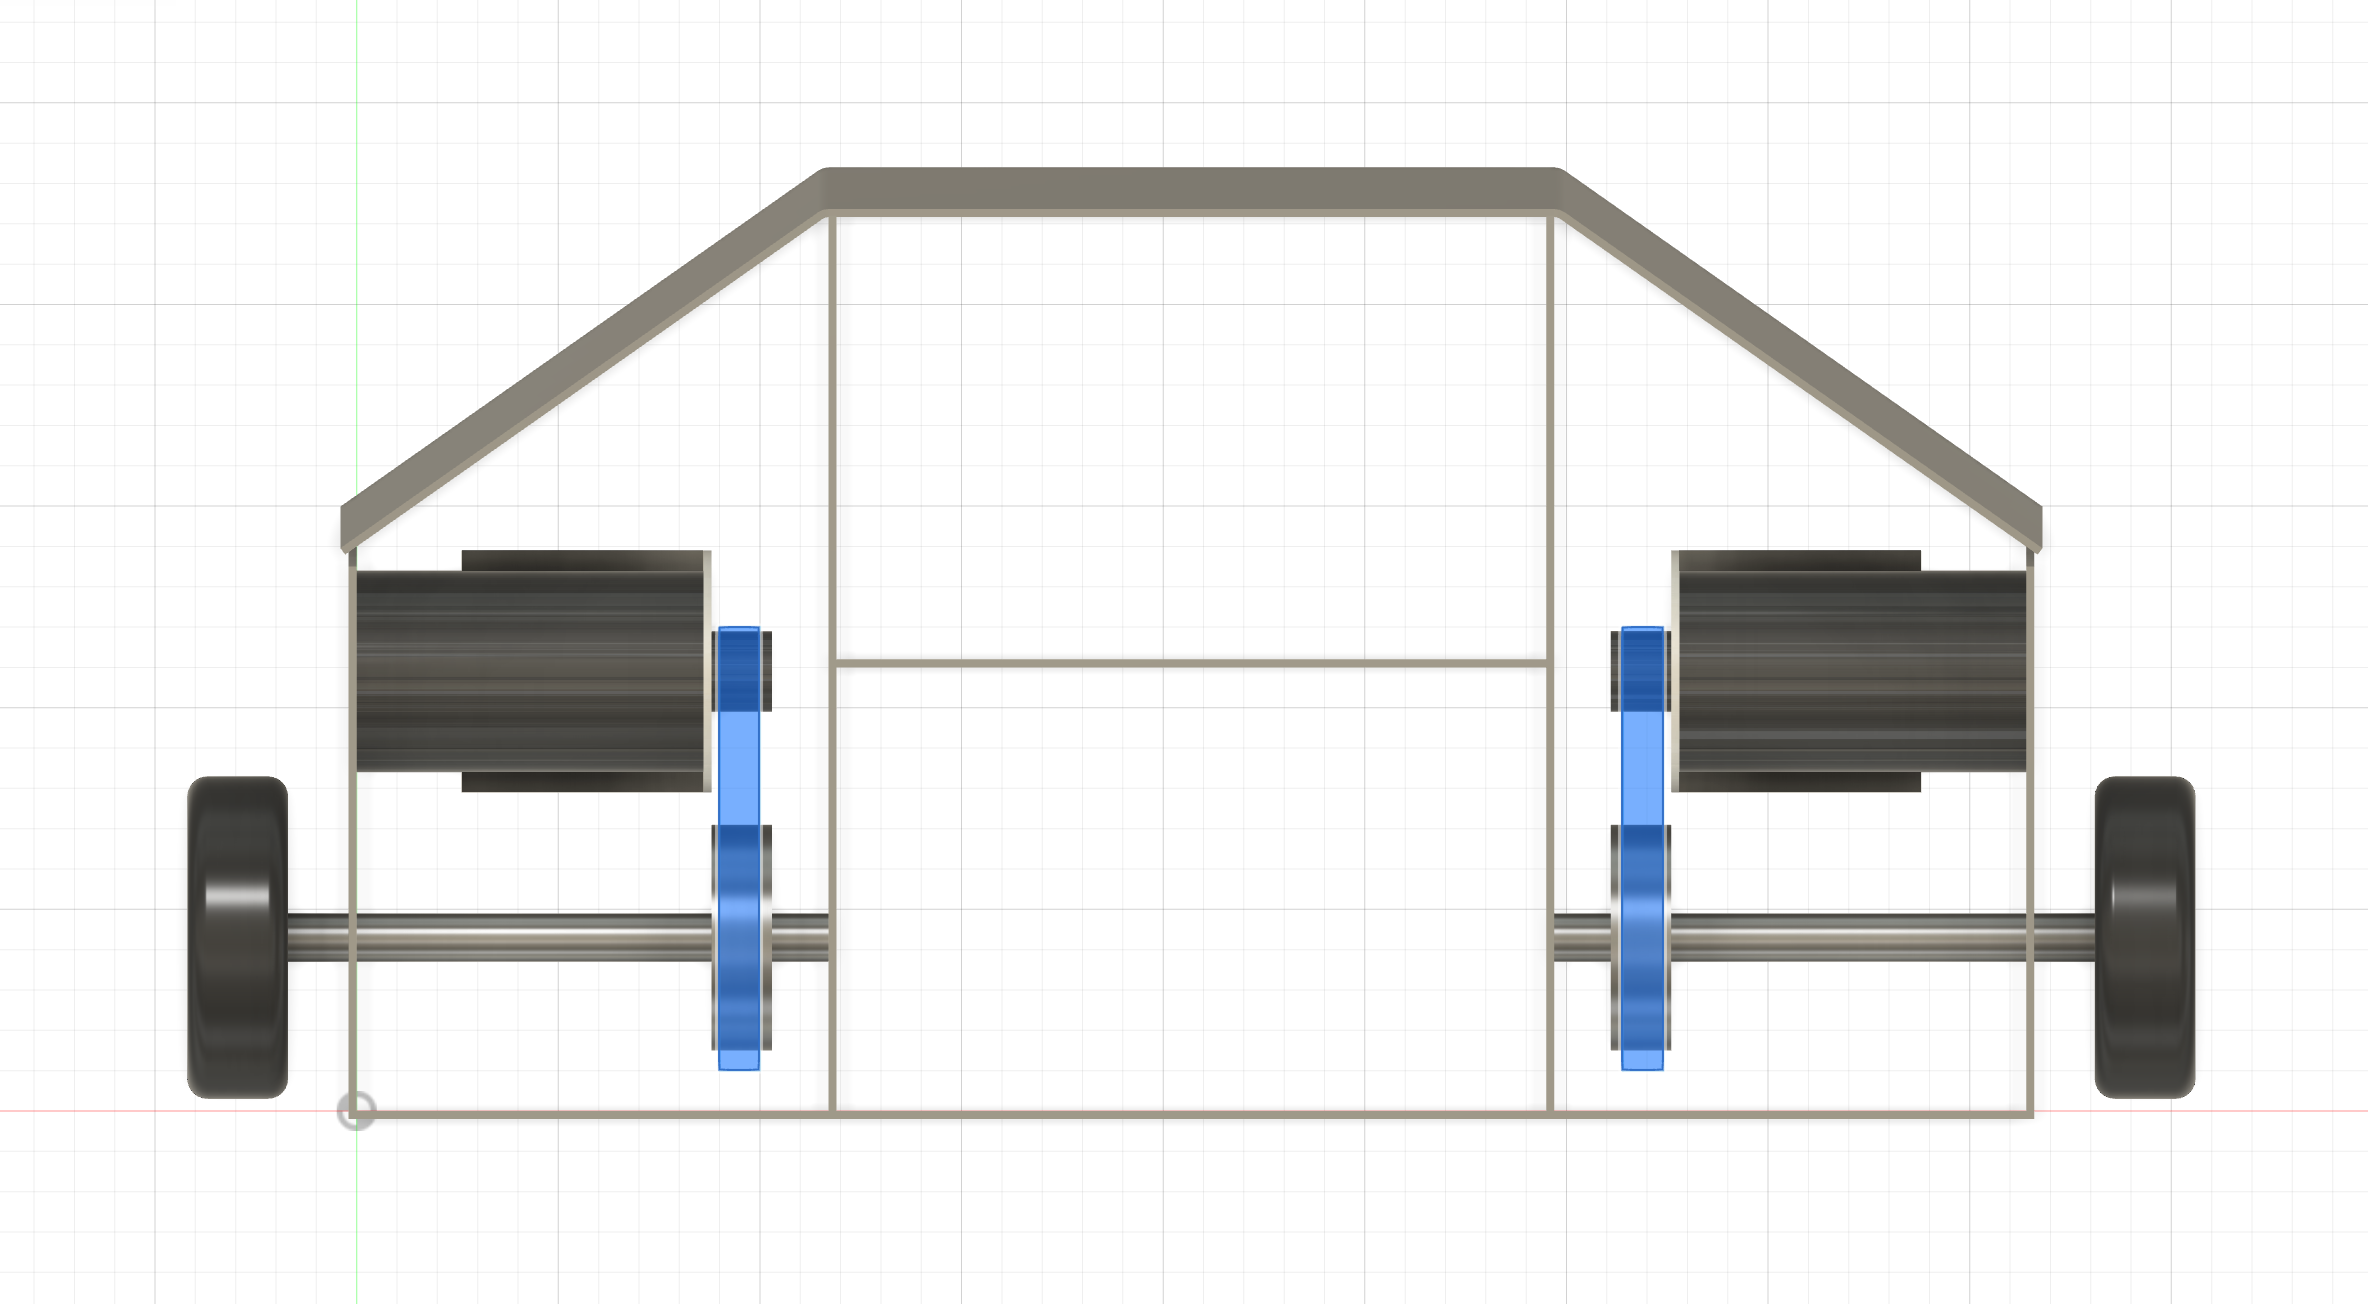
\includegraphics[width=\linewidth]{images/motion.png}
    
    \caption{Схема на задвижването на бойния робот}
    \label{fig:motion} 
\end{figure}

За да може батълбота, който тежи приблизително 18kg, да се задвижва от две колела трябва да бъде пресметнато какъв въртящ момент трябва да достига до всяко от тях
\footnote{Изчисленията са извършени като се приема, че роботът се движи на равна повърхност}
. За целта на изчисленията приемаме, че двете активни колела ще понасят цялото тегло на робота. Понеже на двете колела лежи тежестта от 18kg, означава, че всяко колело изпитва натиска от 9kg или еквивалентните им 88,29N. Коефициента на триене между колелата и пода на арената варира между 0,75 когато робота е в покой и 0,65 когато е в движение. Следователно най-голямата сила на съпротивление, която всяко колело може да генерира без самото колело да се върти е 88,29N х 0.75 = 66,2175N. След като диаметъра на колелото е 80мм следва, че радиусът му е 40мм или 0,04м. Следователно минималният въртящ момент, който позволява на колелата да се въртят е равен на 66,2175N x 0,04m = 2,6487Nm. Следователно минималният въртящ момент, който мотора трябва да достави на колелото е 2,6487Nm, но по време на въртенето си той има само 0,735Nm.

Поради тази причина се налага да се направи редукция на скоростта на мотора за да се увеличи неговия въртящ момент. За да се изчисли каква трябва да бъде нужната редукция трябва да се намери отношението на необходимият въртящ момент и този, който може да бъде генериран. Редукцията, която се получава, че трябва да бъде реализирана между мотора и колелото е минимум 2,6487Nm / 0,735Nm = 3,6.

Начинът, по който е реализирано диференциалното задвижване е като всяко от активните колела бива задвижвано от различен мотор. Връзката между тях е реализирана, чрез зъбчат ремък с ширина 10мм. За да се постигне необходимата редукция, отношението на зъбите на ремъчните ролки на осите на колелата и тези на моторите трябва да бъде равно на нея. Поради това използваните ролки на моторите са с по 10 зъба, а другите са с по 36 зъба. С цел намаляване на триенето между осите на колелата и стените, осите са захванати с лагери в специално изработените за целта лагерни опори, закрепени за стените.

%================================================================================
% РЪКАТА

\section{Задвижване на ръката}

Първата специфична функционалност на разработения боен робот е начина, по който механичната ръка се върти около оста си и се задържа на позицията, на която и бива зададено да седи. Тази задача бива изпълнена чрез употребата на стъпков мотор Nema 24.

За да може ръката да се върти около оста си първо трябва да бъде изчислено какъв въртящ момент ще бъде необходим за целта. Тежестта на ръката е приблизително 4kg, което означава, че силата която е нужно да бъде приложена за да може тя да се завърти е 39,24N. За да пресметнем колко е необходимият въртящ момент за нейното завъртане е необходимо получената сила да бъде умножена по дължината на ръката, която е 240мм(0,24м). По този начин получаваме, че трябва да бъдат приложени 39,24N х 0,24м = 9,4176Nm. Употребеният стъпков мотор може да задържа на една позиция само товари, които изискват въртящ момент 3,1Nm или по-малко, от което следва, че се налага да бъде приложена минимална редукция от 3,03 за да може да бъде реализирано въртенето на ръката.

\begin{figure}[H]
    \centering
    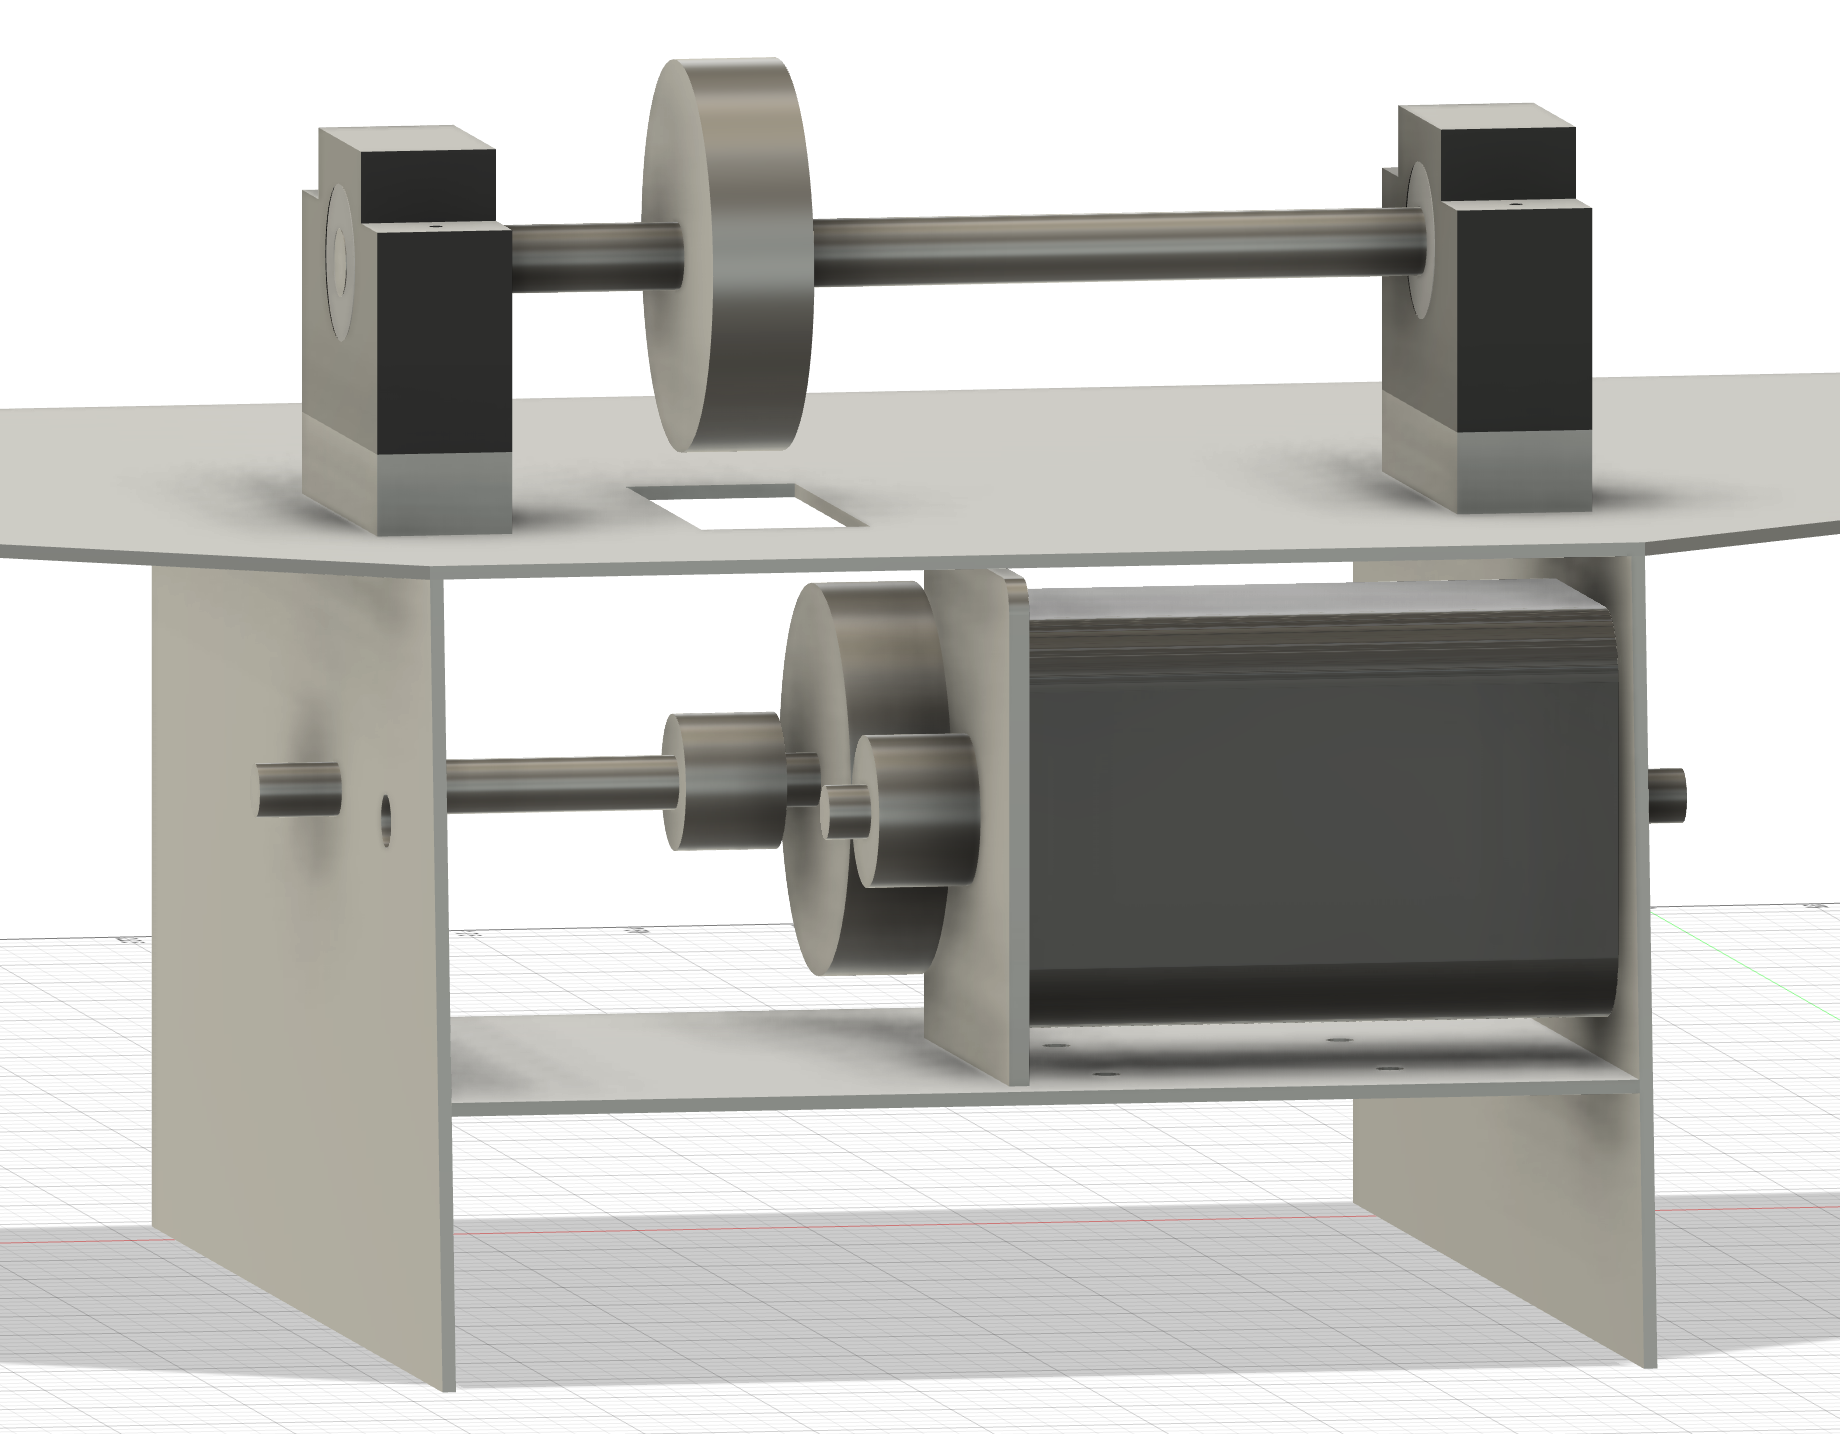
\includegraphics[width=\linewidth]{images/hand-movement.png}
    
    \caption{Схема на задвижването на механичната ръка}
    \label{fig:hand-movement} 
\end{figure}

Начинът, по който е осъществено завъртането на ръката е като тя бива захваната за своята ос така, че чрез завъртането на оста ръката да бъде придвижена заедно с нея. Предаването на движението от стъпковия мотор към оста на ръката е постигнато посредством зъбни ремъци. С цел максималното увеличение на приложената редукция е поставена спомагателна ос между мотора и оста на ръката. По този начин се получават две редукции на движението на мотора. Първата бива от мотора към спомагателната ос, като поставената ролка на мотора има 12 зъба, а тази на спомагателната ос 36 зъба. Постиганата редукция чрез тази връзка е 3. Втората редукция бива от спомагателната ос към оста на ръката и използваните ролки са в същото отношение като тези в предишната предавка. Резултатът от двете връзки е, че общата редукция на скоростта на въртене на мотора се получава да бъде умножението на двете, от които е съставена, което я прави 9. За намаляване на съпротивлението по време на въртенето си са поставени лагерни опори в краищата на двете оси.


%================================================================================
% ОРЪЖИЕТО

\section{Задвижване на оръжието}

Друг проблем, който трябва да бъде решен по време на проектирането на механиката на всеки боен робот е по какъв начин неговото оръжие ще се задвижва. Както е описано в точка \cref{sec:block-schemas} оръжието, което се използва в разработения проект е 180-милиметров диск с ширина 8мм и специфична форма. Формата на диска може да бъде видяна на фигура \cref{fig:disk}. Той е захванат за своята ос така, че чрез завъртането на оста и диска да се върти заедно с нея. Използваният мотор за движението на оръжието е CHANCS 895 DC. Начина, по който е реализирано предаването на движението от мотора до оста на диска е посредством плосък ремък. Избран е плосък ремък за тази цел, а не зъбчат поради причината, че при удар ремъка и мотора трябва отведнъж да спрат своето движение, което често може да доведе до прескачане на зъби на зъбчатия ремък и тяхното ронене. В тези ситуации плоския ремък няма да се амортизира по този начин, а само ще се приплъзне леко по своите ролки. Реализирана е и редукция от 5 на скоростта на тази предавка поради високата скорост, с която би се въртял диска. С цел намаляване на съпротивлението по време на въртенето си в краищата си оста на диска е поставен в лагерни опори, които са застопорени за стените на ръката.

\begin{figure}[H]
    \centering
    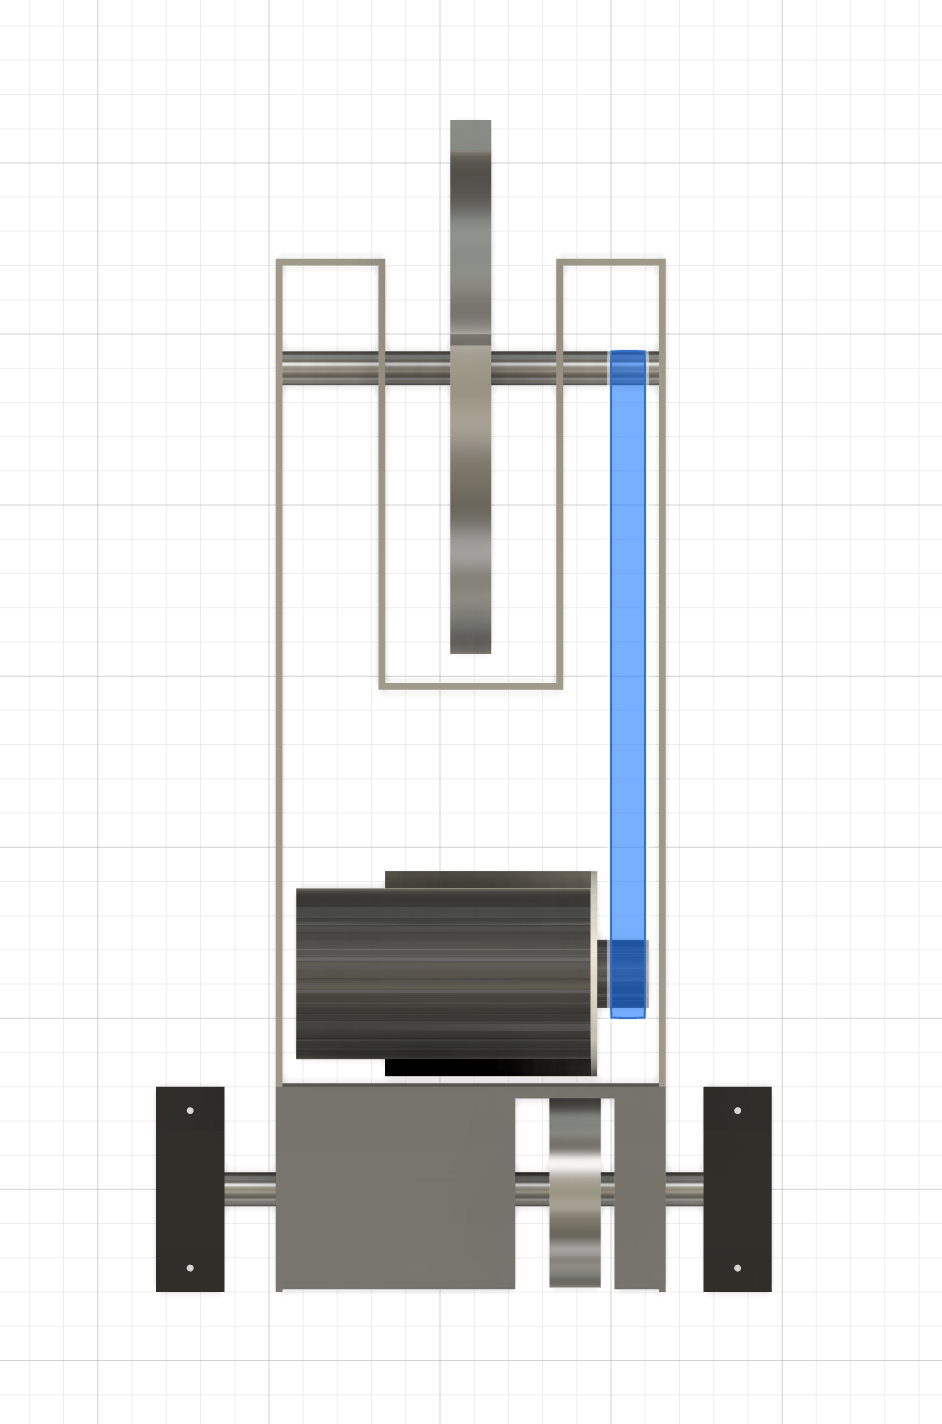
\includegraphics[width=0.8\linewidth]{images/hand-inside.png}
    
    \caption{Схема на задвижването на оръжието}
    \label{fig:hand-inside} 
\end{figure}


\chapter{Проектиране на печатните платки}

За проектирането на печатните платки и монтажните схеми в проекта е използван софтуерния пакет KiCad. Той е избран за целта, защото е безплатен и има богата библиотека с компоненти, съдържащи символи и \textbf{??} очертания на корпуси \textbf{??}.

%================================================================================
% ЕЛЕКТРИЧЕСКА СХЕМА  -  РОБОТ

\section{Принципна електрическа схема на робота}

Принципната електрическа схема на печатната платка в робота може да бъде видяна на \textbf{??} приложение \textbf{??}. Основният елемент на схемата е микроконтролерът STM32F103C8T6 (blue pill), който управлява останалите компоненти. Използваните компоненти в проектирането на тази печатната платка могат да бъдат видяни в таблица \textbf{????} приложение \textbf{????}



\subsection{Радиочестотен модул}

Връзката между дистанционното и робота се осъществява посредством nRF24L01+ PA/LNA радиочестотен модул. Комуникацията между него и използвания микроконтролер е посредством SPI интерфейс. Радиочестотният модул бива захранван с 3,3V от вградения регулатор на напрежението на blue pill. С цел повишаване на съотношението сигнал/шум са поставени 100nF керамичен кондензатор и 100uF електролитен кондензатор, които да намалят съответно високочестотните и нискочестотните шумове.

предавател по далеч / мощни мотори = повече шум
слаб сигнал

+ какво е ПА/ЛНА 
+ режим на СПИ интерфей и неговата скорост
\begin{figure}[H]
    \centering
    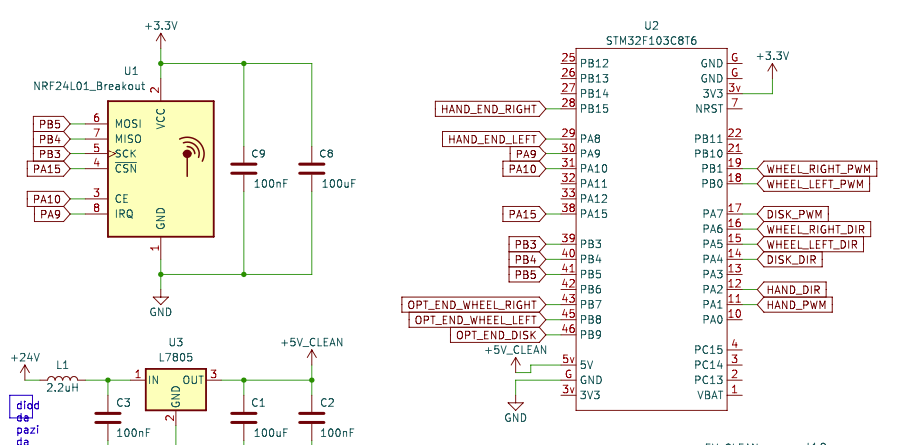
\includegraphics[width=0.6\linewidth]{images/rf-module.png}
    
    \caption{Радиочестотен модул}
    \label{fig:rf-module} 
\end{figure}



\subsection{Управление на моторите}

Управлението на постоянно токовите четкови мотори се извършва посредством MD13S драйвери. Необходимите логически сигнали за да може да се реализира управлението са ШИМ сиганл, който упоменава скоростта, с която мотора трябва да се върти, и високо или ниско ниво, което да показва посоката на движение
\textbf{????}\footnote{Ужасно изказано}.
С цел изолация между микроконтролера и драйверите са поставени оптрони. Начинът на свързване на всеки оптрон може да бъде видян на \cref{fig:brushed-control}. Необходимото захранване на всеки мотор е 24V и то бива подадено посредством отделен конектор.


\begin{figure}[H]
    \centering
    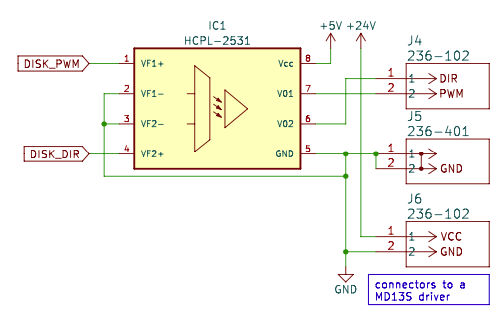
\includegraphics[width=0.6\linewidth]{images/brushed-control.png}
    
    \caption{Оптрон}
    \label{fig:brushed-control} 
\end{figure}


За управлението на стъпковия мотор се използва драйвер DM556T. Сигналите за управление включват ШИМ сигнал, който определя стъпките за изпълнение и логическо ниво (високо или ниско), указващо посоката на движение \textbf{????}\footnote{Ужасно изказано}.
Не е поставен допълнителен оптрон за изолация между драйвера и микроконтролера, поради причината, че на входовете си DM556T има вградени такива. Така направена схемата обаче няма да работи, защото логита на blue pill-а е на 3,3V, докато драйвера използва 5V логика. Този проблем бива решен като се използва преобразувател на логически нива U12, който превежда логическото управление от 3,3V към 5V, съответстващо на логиката, използвана от драйвера.

\begin{figure}[H]
    \centering
    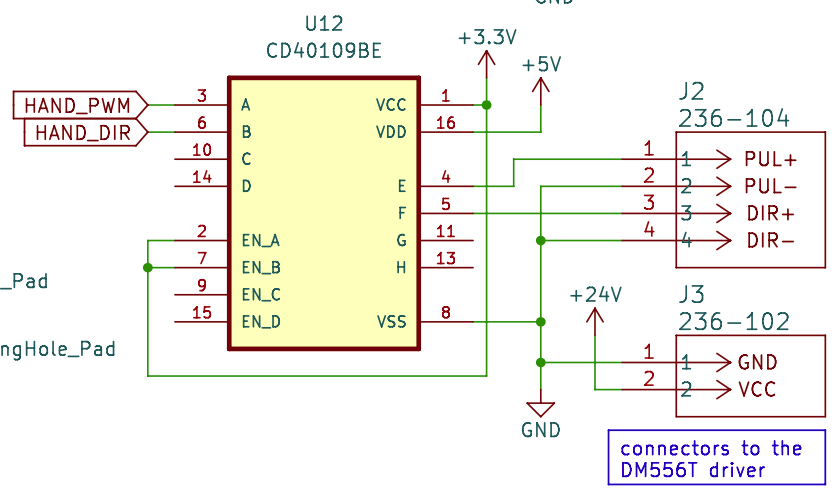
\includegraphics[width=0.6\linewidth]{images/stepper-control.png}
    
    \caption{Левел шифтър}
    \label{fig:stepper-control} 
\end{figure}



\subsection{Сензори}

За следене на скоростта на робота са предвидени и инсталирани оптични сензори. Те биват свързвани към печатната плака чрез конекторите J10, J11 и J12. Всеки сензор има извод за данни и изводи за захранване. 

\begin{figure}[H]
    \centering
    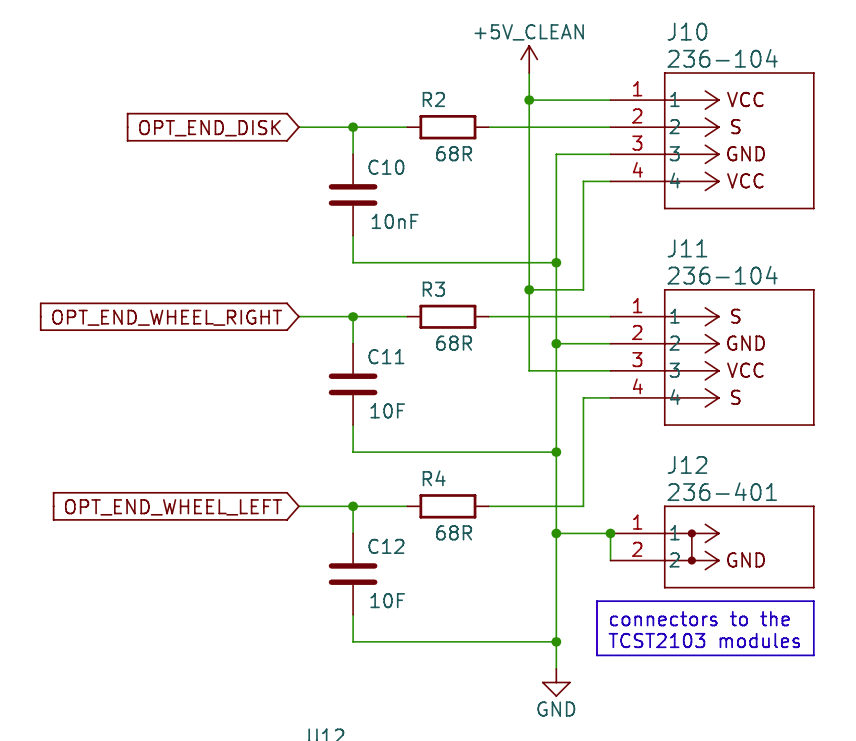
\includegraphics[width=0.6\linewidth]{images/optical-sensors.png}
    
    \caption{оптични сензори}
    \label{fig:optical-sensors} 
\end{figure}

Съгласно изискванията за безопасност са предвидени и крайни изключватели, които да следят дали стъпковият мотор е достигнал някоя от крайните си позиции. Те са свързани, чрез конекторите

\begin{figure}[H]
    \centering
    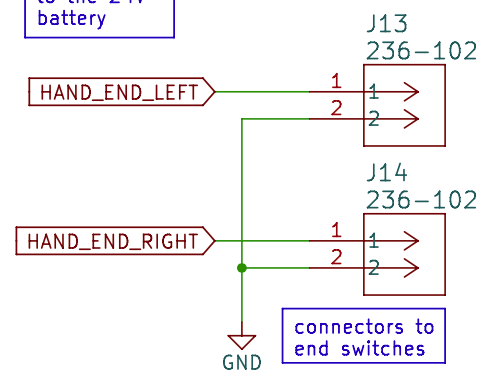
\includegraphics[width=0.6\linewidth]{images/hand-endswitches.png}
    
    \caption{Крайни изключватели за ръката}
    \label{fig:hand-endswitches} 
\end{figure}


\subsection{Захранване на печатната платка}

Печатната платка се захранва директно от 24V постояннотокова батерия. Съгласно изискванията за безопасност изводите на конектор J15 са предвидени за ключ, който да спира цялото захранване на робота. Освен това има имплементирани хардуерни защити против късо съединение, пренапрежение и обратен поляритет на захранването. Първата от трите е реализирана чрез поставянето на автомобилен бушон на държача X1 последователно свързан след главния ключ. Защитата против пренапрежение се осъществява посредством двупосочния трансил D3, който има номинално напрежение \textbf{????}. С цел застраховка против неправилен поляритет на напрежението е поставена P-MOS защита след трансила. Тя се реализира чрез транзистора Q2, ценеровия диод D1 и резистора R1. При правилното свързване на батерията през диода в Q1 протича ток. Поради образувания делител на напрежение D1 и R1, напрежението гейт-сорс на Q2 става равно на пробивното напрежение на D1 и транзисторът се отпушва. В случай, че батерията бъде свързана с обратен поляритет, диодът в Q1 бива свързан в обратна посока и транзисторът остава запушен. 
\textbf{????}\footnote{Стабилизиране на напрежението чрез кондензатора C7}

\begin{figure}[H]
    \centering
    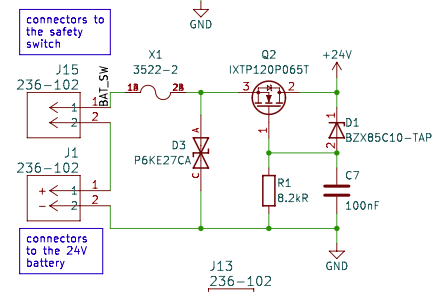
\includegraphics[width=0.6\linewidth]{images/power-protection.png}
    
    \caption{Защити на захранването}
    \label{fig:power-protection} 
\end{figure}

Захранването на логическата част на проекта е постигнато посредством линейни стабилизатори L7805. Tо е разделено на два канала за да може да бъдат намалени шумовете в захранването на микроконтролера и радиочестотния модул \textbf{????}\footnote{Да кажа от къде идват шумовете}. 

Първият канал използва стабилизатора U4 за да успее да свали напрежението до 5V, които да бъдат подадени после на оптроните на логическата част на четковите мотори и на логическия преобразовател на стъпковия мотор. Той е показан на \cref{fig:power-5V}. За намаляване на шумовете в системата са поставени нискочестотния филтър C5 и високочестотния филтър C6. \textbf{????}\footnote{За допълнително стабилизиране на захранването е добавен кондензатора C4 - функция}. 

Вторият канал на захранването е почти идентичен с първия. Той се използва за захранването на микроконтролера, радиочестотния модул и сензорите в робота и може да бъде видян на \cref{fig:power-5V-clean}. \textbf{????}\footnote{бобината L1}.
+две захранвания не два канала
\begin{figure}[H] 
    \centering
    \begin{subfigure}[h]{0.6\textwidth}
        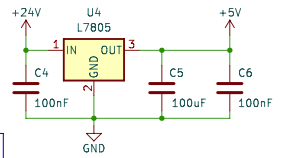
\includegraphics[width=\textwidth]{images/power-5V.png}
        \caption{Захранване на логиката на силовата електроника}
        \label{fig:power-5V}
    \end{subfigure}
    \\ %add desired spacing between images, e. g. ~, \quad, \qquad, \hfill etc. 
      %(or a blank line to force the subfigure onto a new line)
    \begin{subfigure}[h]{0.75\textwidth}
        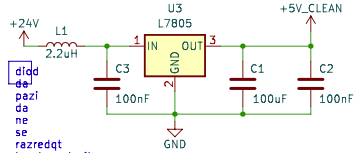
\includegraphics[width=\textwidth]{images/power-5V-clean.png}
        \caption{Захранване на микроконтролера, радиочестотния модул и сензорите}
        \label{fig:power-5V-clean}
    \end{subfigure}
    ~ %add desired spacing between images, e. g. ~, \quad, \qquad, \hfill etc. 
    %(or a blank line to force the subfigure onto a new line)    
    \caption{Захранване на логическата част в робота.}
    \label{fig:power-low}
\end{figure}

%================================================================================
% PCB layout  -  РОБОТ

\section{Опроводяване на печатната платка на робота}

%================================================================================
% МОНТАЖНА СХЕМА  -  РОБОТ

\section{Монтажна схема на робота}

Монтажната схема на робота може да бъде намерена в \textbf{??} приложение \textbf{??}. На нея може да се види основната част в робота, представляваща разработената печатна платка, която съдържа радиочестотния модул за комуникация, микроконтролера, управляващ робота, и хардуерните защити на захранването. Нейното захранване индва от 24V батерия DeWalt DE0241 и съгласно изисканията за безопасност във всеки момент то може да бъде прекъснато чрез ключът SW1. Разработената платка захранва и управлява 3 постояннотокови четкови мотори с помощта на драйвери MD13S. С цел мониторинг на тяхната скорост е предвидено на всеки от тях да има монтиран по един оптичен сензор за скорост. Използваният nema 24 стъпков мотор се управлява посредством DM556T драйвер. Начинат на свързване на драйвера към печатната платка е конфигурация общ катод. Съгласно изискванията за безопасност чрез SW1 и SW2 се следи дали стъпковият мотор не е стигнал до крайните си състояния.

+ параметри на входовете на драйверите

%================================================================================
% ЕЛЕКТРИЧЕСКА СХЕМА  -  ДИСТАНЦИОННО

\section{Принципна електрическа схема на дистанционното}

Принципната електрическа схема на печатната платка на дистанционното може да бъде видяна на \textbf{??} приложение \textbf{??}. Основният елемент на схемата е микроконтролерът STM32F103C8T6 (blue pill), който чете данните от сензорите, обработва ги и после ги праща към робота посредством радиочестотния модул. Използваните компоненти в проектирането на тази печатната платка могат да бъдат видяни в таблица \textbf{????} приложение \textbf{????}



\subsection{Радиочестотен модул}

\subsection{Сензори}

%================================================================================
% PCB layout  -  ДИСТАНЦИОННО

\section{Опроводяване на печатната платка на дистанционното}

%================================================================================
% МОНТАЖНА СХЕМА  -  ДИСТАНЦИОННО

\section{Монтажна схема на дистанционното}

\textbf{????}\footnote{Трябва ли да има такова нещо изобщо}

\chapter{Софтуерна реализация}
\label{chap:software}
% TODO: ask Garistov if 1/4 sec is enough for magic smoke to appear
% TODO: ask Garistov what to do with the messed up interupts
Използваната среда за разработка на софтуерната част от дипломния проект е софтуерния пакет STM32CubbeIDE на STMicroelectronics. Тази платформа е предназначена за изграждане на софтуерното управление на STM микроконтролери и микропроцесори. Чрез интеграцията на GNU GCC компилатор и GBD дебъгер, тя предоставя стабилна среда за разработка на C/C++ програми. В STM32CubbeIDE е интегриран и графичния инструмент STM32CubeMX. Той улеснява конфигурацията и инициализацията на различни части и периферии на микроконтролерите, сред които са пинове, таймери, системни прекъсвания и DMA \textbf{????}\footnote{Превод?}. Друга основна характеристика на избраната среда за разработка е възможността за comprehensive/advanced дебъгинг \textbf{????}\footnote{Превод?} чрез мониторинг на процесорните ядра, регистрите на периферията, паметта и заделените променливи и други. Софтуерният пакет може да бъде свален безплатно от сайта на STMicroelectronics за 64-битовите версии на операционните системи Windows, Linux и macOS. Поради споменатите причини тази среда за разработка беше използвана за проекта.


%================================================================================
% ЛОГИЧЕСКА СХЕМА  -  РОБОТ

\section{Логическа схема на проекта}
\label{sec:logic-schemas}

Съгласно заданието на дипломния проект разработеният боен робот бива управляван посредством специално изработено дистанционно. Комуникацията между тях бива реализирана посредством радиочестотните модули nRF24L01 на компанията Nordic. Те използват вградения си протокол за комуникация Enhanced ShockBurst, който е предназначен за лесна комуникация с ниска енергийна консумация.

Като се получи захранване микроконтролера и радиочестотния модул в дистанционното биват инициализирани. След това започва непрекъснато повтарящият се на равни интерваи цикъл на работа. Първо се прочитат входните данни от потенциометрите и бутоните. След това те биват обработени и записани в подходящ вид. В края на този цикъл обработените потребителски команди биват записани в пакет с инструкции за контрол на бойния робот и той бива изпратен към батълбота за изпълнение. После цикъла на работа на дистанционното започва да се изпълнява отначало. Микроконтролерът е настроен да може да бъдат изпращани по 20 пакета с команди в секунда. Това скорост гарантира на пилота възможността да може да управлява своята машина с минимално системно забавяне.

\begin{figure}[H]
    \centering
    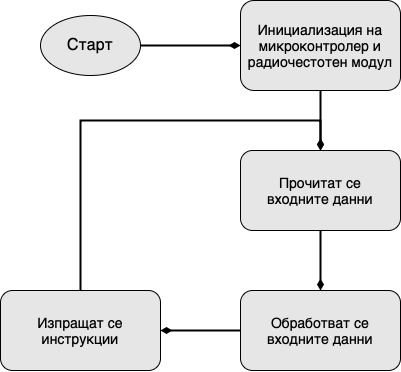
\includegraphics[width=0.6\linewidth]{images/logic-schema-controller.png}
    
    \caption{Логическа схема на дистанционното}
    \label{fig:logic-controller} 
\end{figure}

Полетата, които се съдържат в изпратения пакет са инструкция за позицията, на която трябва да застане механичната ръка на робота, инструкции за скоростта и посоката на въртене на двете колела и инструкция за това дали оръжието трябва да се върти. Структурата на такъв пакет може да бъде видяна на \autoref{lst:payload}.

\lstinputlisting[language=c, consecutivenumbers=false, linerange={11-17}, caption={Пакет инструкции}, label={lst:payload}]{documents/rf-library/NRF24L01.h}

Подобно на дистанционното първата работа на печатната платка, когато получи захранване е да се инициализират микроконтролера и радиочестотния модул. След това започва непрекъснат цикъл на проверяване дали има получен пакет инструкции и ако има се прави опит той да бъде достъпен. При успешното им прочитане те биват заредени в паметта на платката и биват изпълнени. След тази стъпка следва повторно започване на работния цикъл на робота. В случаите, в които няма получени инструкции или не бъде успешно тяхното прочитане, цикъла на работа започва отначало и се спира движението на робота.

\begin{figure}[H]
    \centering
    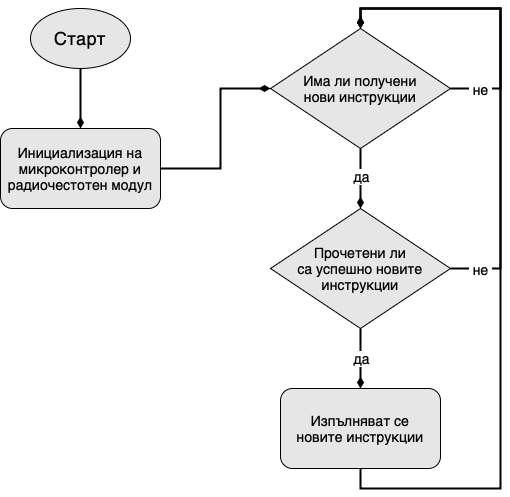
\includegraphics[width=0.6\linewidth]{images/logic-schema-robot.png}
    
    \caption{Логическа схема на робота}
    \label{fig:logic-robot} 
\end{figure}


%================================================================================
% СОФТУЕР  -  РАДИО

\section{Софтуерна реализация на библиотеката на радиочестотния модул}
\label{sec:library}

Безжичната комуникация между дистанционното и бойния робот се осъществава посредством радиочестотния модул nRF24L01 на компанията Nordic. За целите на дипломния проект не беше употребявана готова библиотека за управление на избрания модул, а беше разработена собствена такава. За нейната реализация са употребявани функционалностите на вградената HAL библиотека. С цел улеснение на написването на библиотеката, в заглавния файл са дефинирани като макроси адресите в паметта на регистрите и SPI командните думи. За да може библиотеката да работи, предварително трябва да бъде конфигуриран SPI интерфейса и пиновете, които се използват nRF модула. С цел улеснение на работата с библиотеката е предвидено предварително изводите на радиочестотния модул да имат зададени потребителските етикети NRF24L01\_CSN, NRF24L01\_CE и NRF24L01\_IRQ на съответните им пинове на микроконтролера.

Основните функционалности, които трябва да бъдат реализирани, за да може библиотеката да бъде разработена са писане и четене на регистрите на радиочестотния модул. За да се пише в регистър се подготвя масив с дължина 2 байта. В първия се поставя номера на регистъра, а във втория стойността, която трябва да бъде записана. За да може nRF модула да разбере, че трябва да запише получената стойност, трябва да бъде поставена единица на 5-та позиция от първия байт. Съгласно секция 8.3. "SPI комуникация" от документацията на nRF24L01 всяка SPI операция трябва да бъде започната с падащ фронт на CSN извода на радиочестотния модул. След това се извиква HAL функцията за предаване на информация по SPI интерфейса.

\lstinputlisting[language=c, consecutivenumbers=false, linerange={37-51}, caption={Писане в регистър}, label={lst:write-register}]{documents/rf-library/NRF24L01.c}

Четенето на регистър се реализира аналогично. При него не се подготвя масив, в който да се постави адреса на регистъра и той не бива редактиран. Вместо това първо се използва HAL функцията за предаване на номера на регистъра, който трябва да бъде прочетен, и след това се използва HAL функцията за получаване на данни по SPI.

\lstinputlisting[language=c, consecutivenumbers=false, linerange={72-87}, caption={Четене на регистър}, label={lst:read-register}]{documents/rf-library/NRF24L01.c}

Основната част от регистрите в паметта на използвания nRF модул са с размер 1 байт, но тези, които съхраняват адреси за каналите за комуникация 0 и 1 имат 5 пъти по-голяма дължина. Поради тази причина са написани функциите nrf24\_write\_reg\_multi() и nrf24\_read\_reg\_multi(), които съответно могат да бъдат видени на \autoref{lst:write-big-register} и \autoref{lst:read-big-register}. Те са реализирани аналогично на по-малките им подобни функции.

\lstinputlisting[language=c, consecutivenumbers=false, linerange={52-70}, caption={Писане на големи регистри}, label={lst:write-big-register}]{documents/rf-library/NRF24L01.c}

\lstinputlisting[language=c, consecutivenumbers=false, linerange={88-99}, caption={Четене на големи регистри}, label={lst:read-big-register}]{documents/rf-library/NRF24L01.c}


%================================================================================
% ИНИЦИАЛИЗАЦИЯ

\subsection{Инициализация на модула}
\label{ssec:init}

При получаване на захранване първата задача на микроконтролера и радио модула е да бъдат конфигурирани. Инициализацията на първия може да бъде видяна в \cref{ssec:init-controller} и \cref{ssec:init-robot}. Привеждането на радиочестотния модул в състояние, което позволява безжично предаване на информация е осъществено като се извикват една след друга първо функцията за инициализация на модула и след това и допълнителна такава, с която се пояснява дали същия е предавател или получател на информацията.

При началото на инициализацията на CE пина се подава ниско ниво за да се гарантира, че няма да се активира механизма за изпращане на данни. След това се подават зануляват стойностите на CONFIG и RF\_CH регистрите. Те следва да бъдат редактирани при задаването на роля на модула(предавател или приемник). Чрез записване на 0 в EN\_AA регистъра се изключват автоматичните потвърждения по време на безжичното предаване. В регистъра EN\_RXADDR стойността 0 спира употребата на 6-те информационни канала. За да се дефинира дължината на адреса да бъде 5 байта в регистъра SETUP\_AW са поставени единици на битове 0 и 1. Последния регистър, който се конфигурира в рамките на тази функция е RF\_SETUP. Чрез поставяне на 0 на 3 бит в него се задава скоростта на предаване на информация да бъде 1Mbps, а посредством единици на битове 1 и 2, мощността на предаване на изхода на радиото е 0dBm. 

\lstinputlisting[language=c, consecutivenumbers=false, linerange={145-159}, caption={Инициализация на радио модула}, label={lst:init}]{documents/rf-library/NRF24L01.c}

След функцията за инициализиране на nRF модула се извиква функция, която да пояснява дали модула е предавател или получател на данни. В \autoref{lst:conf-transmitter} може да бъде видяна процедурата за конфигуриране предавател. Първо се задава в регистър RF\_CH честотата (канала), на която ще се предава информацията. След това се записва 5 байтовия адрес на получателя в TX\_ADDR регистъра. После без да се редактира останалата част от регистъра в CONFIG се поставят единица на бит 1 и се оставя нула на бит 0 съответно за да се стартира дейността на радиочестотния модул и за да се влезе в режим на изпращач на информация. 

\lstinputlisting[language=c, consecutivenumbers=false, linerange={164-174}, caption={Конфигуриране на изпращач на данни}, label={lst:conf-transmitter}]{documents/rf-library/NRF24L01.c}

Подобно на последно разглежданата функция NRF24\_RX\_mode() започва със задаване на честотата на предаване на информация. След това без да се редактира останалата част от регистъра EN\_RXADDR се поставя единица на бит 1 поради за да се позволи употребата на информационен канал 1. После се записва 5 байтовия адрес на изпращача на информация в RX\_ADDR\_P1 регистъра. За да се дефинира дължината на пакета данни, който ще се изпраща безжично, се записва големината на структурата Payload в регистъра RX\_PW\_P1. След това без да се реактира останалата му част в CONFIG регистъра се поставят единици на битове 0 и 1 съответно за да се стартира дейността на радиочестотния модул и за да се влезе в режим на получател на данни. В края на тази функция CE пина бива поставен във високо състояние и се държи в това през целия период на работа. В случай, че CE мине в ниско ниво, nRF модула ще излезе от режима на получател.

\lstinputlisting[language=c, consecutivenumbers=false, linerange={234-256}, caption={Конфигуриране на получател на данни}, label={lst:conf-receiver}]{documents/rf-library/NRF24L01.c}

Стойностите, които са избрани за скорост на безжичното предаване, мощността на предаване на изхода на nRF модула и честотата на излъчване на сигнали са подбрани такива, че да осигуряват максимален обхват на безжичната комуникация.

%================================================================================
% ИЗПРАЩАНЕ НА ДАННИ

\subsection{Изпращане на информация}
\label{ssec:transmit}

Изпращането на пакет инструкции от дистанционното към робота се извършва посредством функцията NRF24\_transmit(). Първата стъпка от нейното изпълнение е пакета с инструкции да бъде зареден в паметта на радио модула, посредством функцията, която може да бъде видяна в \autoref{lst:push-payload}. След това се генерира импулс на CE извода по-дълъг от 10us. Съгласно секция 6.1.5. "режим предаване" от документацията на nRF24L01 при такъв импулс в режима за изпращане на данни, записаните в паметта на модула пакети инструкции започват да се излъчват. Останалата част на функцията проверява дали пакетите са били изпратени успешно като проверява съдържанието на FIFO\_STATUS регистъра. Ако четвъртият бит в него е вдигнат означава, че пакета е бил успешно изпратен.

\lstinputlisting[language=c, consecutivenumbers=false, linerange={204-228}, caption={Изпращане на пакет инструкции}, label={lst:transmit}]{documents/rf-library/NRF24L01.c}

Когато се зарежда пакет инструкции в паметта на радиочестотния модул, първо се проверява дали пакета не е твърде голям. В случай, че е опита за безжично изпращане на инструкциите бива прекратен. Останалата част от зареждането на пакета наподобява значително функциите за писане в регистри. Първо се заделя масив от еднобайтови променливи. След това на първа позиция в масива се записва SPI командата за записване на пакета в паметта на модула и чрез функцията memcpy() се записва съдържанието на пакета в масива от втория елемент нататък. Както беше споменато в предишната секция следва да се направи падащ фронт на пин CSN. Когато буфера е вече готов, той бива зареден в паметта, чрез HAL функцията за предаване на информация по SPI интерфейса. Накрая функцията завършва като CSN пина ве върне в свойто предишно състояние.

\lstinputlisting[language=c, consecutivenumbers=false, linerange={175-202}, caption={Зареждане на пакет инструкции}, label={lst:push-payload}]{documents/rf-library/NRF24L01.c}

%================================================================================
% ПОЛУЧАВАНЕ НА ДАННИ

\subsection{Получаване на информация}
\label{ssec:receive}

Получаването на пакети с инструкции се реализира чрез две функции. Първата проверява дали има нова получена информация в радио модула, а втората е същинското и извличане в паметта на микроконтролера. Проверката се осъществява като се прочита STATUS регистъра. Ако бит 6 е единица следва, че има получени нови команди, а в битове 1, 2 и 3 е запазен номера на информационния канал, от който е получената информация. След това стойността на същия регистър се рестартира и функцията връща резултат, показващ, че има получени данни. 

\lstinputlisting[language=c, consecutivenumbers=false, linerange={256-273}, caption={Проверка дали има получен пакет инструкции}, label={lst:check-delivered}]{documents/rf-library/NRF24L01.c}

Във функцията за извличане на данни първата първо се дефинират двата помощни масива. В първия се записва SPI командата R\_RX\_PAYLOAD, която се използва за да се извлече получения нов пакет информация, а във втория следва тя да се бъде записана. След това посредством HAL функцията за предаване и получаване на информация по SPI интерфейса командата се изпраща до радиочестотния модул и сеполучава резултата във втория помощен масив. После чрез функцията memcpy() информацията се премества от помощния регистър в желаната променлива.

\lstinputlisting[language=c, consecutivenumbers=false, linerange={275-299}, caption={Получаване на пакет инструкции}, label={lst:receive}]{documents/rf-library/NRF24L01.c}



%================================================================================
% СОФТУЕР  -  ДИСТАНЦИОННО

\section{Софтуерна реализация на дистанционното}
\label{sec:software-controller}

Както e описано в \cref{sec:block-schemas} компонентите, които се използват в дистанционното са 2 потенциометъра и 3 бутона.

%================================================================================
% ИНИЦИАЛИЗАЦИЯ

\subsection{Инициализация на микроконтролера на дистанционното}
\label{ssec:init-controller}

След като получи захранването си микроконтролера преминава през серия от процеси, които трябва да конфигурират използваните периферии, изводи и променливи. Посредством функцията HAL\_Init() се рестартират всички периферии и се инициализират HAL библиотеката и всички нейни функционалности. След това чрез SystemClock\_Config() се конфигурира системния таймер. После следва конфигурацията на изводите на микроконтролера. Една от тях може да бъде видяна в \autoref{lst:conf-pin-controller}. За това кой пин как е конфигуриран и за какво се използва може да се разбере от таблица \cref{table:pins-controller}. След това се инициализира SPI връзката с nRF модула. Чрез MX\_TIM4\_Init() се инициализира таймер 4, с помощта на когото се изпращат пакетите с инструкции на равни периоди. След това се инициализират и двата аналогово-цифрови преобразувателя, които се използват за четене на състоянието на потенциометрите. Последната инициализация е тази на радиочестотния модул и се задава неговия режим на работа. Преди да започне повтарящият се цикъл на работа таймера се стартира и се пуска калибрация на аналогово-цифровите преобразуватели.

\lstinputlisting[language=c, consecutivenumbers=false, linerange={72-76}, caption={Конфигуриране на пин}, label={lst:conf-pin-controller}]{documents/controller/gpio.c}

\begin{table}[H]
    \centering
    \begin{tabular}{| m{4cm} | m{3,5cm} | m{3,5cm} | m{3,5cm} |}
        \hline
        & Wi-fi & Bluetooth & nRF24L01+ \\
        \hline
        Скорост &  Висока & Средно & Средна \\
        \hline
        Обхват & 10ки метри & 10 метра & 10-150 метра \\
        \hline
        Енергийна консумация & Висока & Средна & Ниска\\
        \hline
    \end{tabular}
    \caption{Пинове}
    \label{table:pins-controller}
\end{table}

%================================================================================
% РАБОТЕН ЦИКЪЛ

\subsection{Работен цикъл на дистанционното}
\label{ssec:loop-controller}

Както е описано в \cref{sec:logic-schemas} цикъла на работа се повтаря на равни интервали. Това е постигнато посредством прекъсването при преливане на таймер 4. Той е конфигуриран така, че прекъсването да бъде генерирано на всяка десета от секундата. След извикването на прекъсването се вдига флага send\_flag. При това действие се прочитат състоянията на потенциометрите и се записват на полетата за скорост на лявото и дясното колело. Това е последвано от извикването на функцията за калибриране на данните. В края на този цикъл се инициира изпращане на пакета с инструкциите и при успех се сменя състоянието на вградения светодиод.

\lstinputlisting[language=c, consecutivenumbers=false, linerange={113-134}, caption={Работен цикъл}, label={lst:loop-controller}]{documents/controller/controller.c}

Успоредно на това има конфигурирани и външни прекъсвания. Те имат функцията да редактират позицията на ръката и да пускат или спират движението на оръжието.




%================================================================================
% СОФТУЕР  -  РОБОТ

\section{Софтуерна реализация на управлението на робота}
\label{sec:software-robot}

%================================================================================
% ИНИЦИАЛИЗАЦИЯ

\subsection{Инициализация на микроконтролера на робота}
\label{ssec:init-robot}

След като получи захранването си микроконтролера преминава през серия от процеси, които трябва да конфигурират използваните периферии, изводи и променливи. Посредством функцията HAL\_Init() се рестартират всички периферии и се инициализират HAL библиотеката и всички нейни функционалности. След това чрез SystemClock\_Config() се конфигурира системния таймер. После следва конфигурацията на изводите на микроконтролера. Една от тях може да бъде видяна в \autoref{lst:conf-pin-robot}. За това кой пин как е конфигуриран и за какво се използва може да се разбере от таблица \cref{table:pins-robot}. След това се инициализира SPI връзката с nRF модула. Чрез функциите MX\_TIM3\_Init(), MX\_TIM2\_Init() и MX\_TIM4\_Init() се инициализират таймери 2, 3 и 4. Таймер 3 се използва за генериране широчинно импулсен сигнал за контролиране на скоростта на въртене на четковите мотори, а 4-тия се използва за измерване на тяхната скорост. Таймер 2 се използва за генерирането на импулси за движението на робота. След това се инициализира радиочестотния модул и се задава неговия режим на робота. Чрез функцията HAL\_TIM\_PWM\_Start() се стартира генерирането на широчинно импулсния сигнал. Преди да започне повтарящият се цикъл на работа и таймери 2 и 4 се стартират.

\lstinputlisting[language=c, consecutivenumbers=false, linerange={72-76}, caption={Конфигуриране на пин}, label={lst:conf-pin-robot}]{documents/controller/gpio.c}

\begin{table}[H]
    \centering
    \begin{tabular}{| m{4cm} | m{3,5cm} | m{3,5cm} | m{3,5cm} |}
        \hline
        & Wi-fi & Bluetooth & nRF24L01+ \\
        \hline
        Скорост &  Висока & Средно & Средна \\
        \hline
        Обхват & 10ки метри & 10 метра & 10-150 метра \\
        \hline
        Енергийна консумация & Висока & Средна & Ниска\\
        \hline
    \end{tabular}
    \caption{Пинове}
    \label{table:pins-robot}
\end{table}

%================================================================================
% РАБОТЕН ЦИКЪЛ

\subsection{Работен цикъл на робота}
\label{ssec:loop-robot}

Както е описано в \cref{sec:logic-schemas} цикъла на работа започва с проверка на това дали има получен нов пакет инструкции. Ако има получен такъв се извиква функцията за извличане на данните от радиочестотния модул и ако е успешна се извиква функцията, която прилага инструкциите.

\lstinputlisting[language=c, consecutivenumbers=false, linerange={122-135}, caption={Работен цикъл}, label={lst:loop-robot}]{documents/robot/robot.c}

Функцията за прилагането на инструкциите е съставена от помощни функции. Първо чрез функцията get\_brushed\_DIR() се проверява в коя посока кой от четковите мотори трябва да се върти и се задава съответната стойност на съответния извод. След това посредством get\_brushed\_DIR() се задава какъв трябва да бъде коефициента на запълване на широчинно-импулсния сигнал, който се използва за дава каква трябва да бъде скоростта на въртене на четковите мотори.

\lstinputlisting[language=c, consecutivenumbers=false, linerange={249-280}, caption={Управление на четковите мотори}, label={lst:dc-motor}]{documents/robot/robot.c}

Последната функция, която се извиква във функцията unload\_payload() се казва get\_hand\_DIR(). Тя се използва за да се определя посоката на движение на стъпковия мотор. Импулсите за колко стъпки да бъдат направени се генерират чрез прекъсването при преливане на таймер 2. Функцията за обработка на прекъсването може да бъде видяна в \cref{lst:overflow-interupts}.

\lstinputlisting[language=c, consecutivenumbers=false, linerange={282-297}, caption={Управление на стъпковия мотор}, label={lst:stepper-motor}]{documents/robot/robot.c}

%================================================================================
% СЕНЗОРИ ЗА ОБРАТНА ВРЪЗКА

\subsection{Сензори за обратна връзка}
\label{ssec:feedback-sensors}

Съгласно изискванията за безопасност описани в \cref{sec:requirements} са имплементирани и двата крайни изключвателя за ръката. Те са свързани към изводи на микроконтролера, за които има конфигурирани външни прекъсвания, които се генерират при падащ и нарастващ фронт на вълната. Когато такова прекъсване се появи се вдига флаг, който спира работата на движението на ръката докато ръката не отвори отново крайния изключвател. 

\lstinputlisting[language=c, consecutivenumbers=false, linerange={184-209}, caption={Външни прекъсвания}, label={lst:external-interupts}]{documents/robot/robot.c}

В проекта има монтирани и оптични сензори, чрез които се следи приблизителната скорост на четковите мотори. Тази функционалност е реализирана посредством външни прекъсвания и прекъсване при преливане. При генерирането на първото се увеличава променлива, която съдържа броя завъртания на съответния мотор. Чрез прекъсването при преливане на таймер 4, на равни интервали от време, се проверява дали има направени завъртания за текущия период. Ако няма направени следва да бъде забранено на съответния мотор да се върти известно време.

\lstinputlisting[language=c, consecutivenumbers=false, linerange={211-247}, caption={Прекъсвания при преливане}, label={lst:overflow-interupts}]{documents/robot/robot.c}




\chapter{Заключение}

%================================================================================
% Съдържание

\tableofcontents
\listoffigures
\listoftables
\printbibliography

\end{document}
